Desirable properties of an MBT are high performance, good interpretability and stability.
In this chapter, simulation scenarios are described with which an empirical comparison of these properties for the different MBT algorithms is carried out.
In addition, a comparison of the performance and interpretability of SLIM MBTs is made when objectives of different complexity are used for modelling.

\subsection{Evaluation measures}
To evaluate the desired properties we use the following definitions and measurements.

\subsubsection{Performance}
A central aspect in the comparison of the different MBT algorithms is their performance. 
To find out how well an MBT algorithm performs as a stand-alone machine learning model, the MBT is fitted to the original response. 
In the following, the mean squared error ($MSE$) and $R^2$ are used as performance measures of accuracy, which are defined as
\begin{align}
    MSE \left( \left\{y, \hat{y}\right\}\right) = \frac{1}{n}\sum_{i = 1}^{n}\left(y^{(i)}-\hat{y}^{(i)}\right)^2
\end{align}
\begin{align}
    R^2\left( \left\{y, \hat{y}\right\}\right) = 1-\frac{\sum_{i = 1}^{n}\left(\hat{y}^{(i) } - y\right)^2}{\sum_{i = 1}^{n}\left(y^{(i)} - \bar{y}\right)^2},
\end{align}
where $\hat{y}^{(i)}, i = 1,...,n$ are the predictions of the MBT model and $\bar{y}$ is the arithmetic mean of the target $y$.

To determine how well the respective MBT algorithm works as a surrogate model, i.e. how well the predictions of a black box model are replicated by the MBT, $MSE(\left( \left\{y^{bb}, \hat{y}\right\}\right)$ and $R^2_{fid}\left( \left\{y^{bb}, \hat{y}\right\}\right)$ are used to measure fidelity. 

Accuracy and fidelity are measured on both training and test data in order to make a statement about the generalisation performance of the MBTs.

\vspace{0.5cm}
\subsubsection{Interpretability}
When evaluating the suitability of an MBT algorithm as a surrogate model, the trade-off between performance and interpretability is the central aspect. While performance is easy to measure, the concept of interpretability is much more abstract.
According to \citet{DoshiVelez.2017} interpretability is defined as the ability to explain or present something to a person in understandable terms. If, for different MBT algorithms to be compared, the models in the leaf nodes are defined as equally complex (e.g. linear regression models), these do not have to be taken into account when comparing interpretability, but only the structure of the tree is relevant. We then use the number of leafnodes as the most important criterion for interpretability.  The underlying assumption is: the fewer leafnodes a tree has, the easier its structure is to understand.

As an additional measure, we include the number of different features used for splitting. The idea here is that the splitting of the feature space is easier to understand if it is done in few dimensions.



\subsubsection{Stability}
A well-known weakness of recursive partitioning algorithms is that the resulting decision trees are often unstable, meaning that slight fluctuations in the training data can lead to large differences in the models \citep{Fokkema.2020}.
Depending on whether differences between two decision trees mean different predictions for the same observations or different structural properties of a tree, such as the number of leaf nodes, we speak of semantic or structural instability \citep{Wang.2018}. 
Since we are looking for MBTs that are easy to interpret, it is not enough to look at semantic stability. It would be desirable for an MBT that has been fitted twice on slightly different training data to partition the feature space in the same way. To compare two trees that have the same number of leafnodes, an additional data set (evaluation data) is used that is clustered according to the decision rules found for the training data. The subregions of an MBT are defined as the clustering of the evaluation data set according to the decision rules learned by fitting the MBT to a training data set. 
If the clustering of the evaluation data is identical for both MBTs, the interpretation of the decision rules is also identical, even if the order of split features in the two MBTs is reversed and the rules therefore appear different at first glance.
In order to measure the similarity of subregions found by MBTs trained on slightly different data we use the Rand index (RI) \citep{Rand.1971}. The RI defines the similarity of two clusterings $\mathcal{A}, \mathcal{B}$ of $n$ observations each by the proportion of  the number of observation pairs that were either assigned to the same partition in both clusterings ($n_{11}$) or to different partitions in both clusterings ($n_{00}$) measured against the total number of observation pairs. 
\begin{align}
    RI(\mathcal{A}, \mathcal{B}) = \frac{n_{11} + n_{00}}{\binom{n}{2}}
\end{align}
\citep{Gates.2017}

The higher the RI for a pair of trees with the same number of leaf nodes, the more similar the subregions defined by these trees and the more stable the MBT algorithm is in a concrete simulation scenario. 


Besides the similarity of subregions with the same number of leafnodes, we use the variability of the number of leafnodes as a measure of stability. The more the number of leaf nodes fluctuates in for an MBT algorithm, the more unstable we consider it to be.

According to \citep{Hu.2020}, the stability problem with SLIM is less if it is used as a surrogate and not as stand-alone model on the original data. However, this is not shown in the paper. Therefore, this claim is empirically investigated here for all MBT Algorithms presented by comparing the stability of MBTs on the original data with the stability of MBTs used as surrogate models.





\subsection{Basic scenarios}
We use three simple scenarios that differ mainly in the type of interaction(s) they contain (smooth interaction vs subgroup depending effects). Based on these scenarios the different MBT algorithms are compared with respect to performance, interpretability and stability.


\subsubsection{Scenarios}
The data generating processes of the basic scenarios are defined as follows:


\paragraph{Linear smooth}
Numerical features with linear effects on y and smooth interactions
\begin{itemize}
    \item $\textbf{x}_1,..., \textbf{x}_{3} \sim U(-1,1)$
    \item $ f_{ls}(\textbf{x}) = \textbf{x}_1 + 4   \textbf{x}_2 + 3   \textbf{x}_2   \textbf{x}_3 $
    \item $\epsilon \sim N(0, 0.1 \cdot sd(f_{ls}(\textbf{x}))$
    \item $y = f_{ls}(\textbf{x}) + \epsilon$
\end{itemize}             


\paragraph{Linear categorical}
Numerical and binary features with linear effects and subgroup specific linear effects
\begin{itemize}
    \item $\textbf{x}_1, \textbf{x}_2 \sim U(-1,1)$, $\textbf{x}_3 \sim Bern(0.5)$,  
    \item $ f_{la}(x) =  \textbf{x}_{1} - 8  \textbf{x}_2 + 16  \textbf{x}_2  \mathbf{I}_{\textbf{x}_3 = 0} + 8  \textbf{x}_2  \mathbf{I}_{\textbf{x}_1 > mean(\textbf{x}_1)} $
    \item $\epsilon \sim N(0, 0.1 \cdot sd(f_{la}(\textbf{x}))$
    \item $y = f_{la}(\textbf{x}) + \epsilon$          
\end{itemize}



The scenario is based on a simulation example in \citep{Herbinger.2022}.

\paragraph{Linear mixed}
Numerical and binary features with linear effects, subgroup dependent and smooth two- and three-way interactions
\begin{itemize}
    \item $\textbf{x}_1, \textbf{x}_2 \sim U(-1,1)$, $\textbf{x}_3, \textbf{x}_4 \sim Bern(0.5)$
    \item $f_{lm}(\textbf{c}) = 4   \textbf{x}_2 + 2   \textbf{x}_4  + 4   \textbf{x}_2   \textbf{x}_1 + 8   \textbf{x}_2   \mathbf{I}_{\textbf{x}_3 = 0} +  8 \textbf{x}_1   \textbf{x}_2 \mathbf{I}_{\textbf{x}_4 = 1}$
    \item $\epsilon \sim N(0, 0.1 \cdot sd(f_{lm}(x))$
    \item $y = f_{lm}(\textbf{x}) + \epsilon$
\end{itemize}



\subsubsection{Simulation Setting}
Since the number of leafnodes and the performance strongly depend on the prepruning value for $impr$ for SLIM and GUIDE and $alpha$ for MOB and CTree, the simulations are carried out for different values of these parameters. In addition, two different sample sizes $n$ are chosen. 
All MBT algorithms are fitted as standalone models on the original data and as surrogate models on a correctly specified linear model or GAM and on an xgboost model with correctly specified interactions. The configurations of the xgboost models are listed in the appendix.
Table \ref{tab:simulation_setting} lists all varied factors and their levels. In total, there are $3 \times 2 \times 3 \times 3 = 54$ variants for each of the 4 MBT algorithms.
Settings that are fixed in all variants are maximum tree depth of $6$ and a minimum node size of $50$.
The experiment is repeated $N = 100$ times.

\begin{table}[!htb] 

\caption{Simulation setting basic scenarios}
\centering \small
\begin{tabular}[t]{lll}
\hline
Varied factors & levels \\
\hline
Scenario  & linear smooth, linear categorical, linear mixed\\
Sample size $n$  & 1500, 7500 ($\frac{2}{3}$  training, $\frac{1}{3}$ test data)\\
Prepruning parameters   & $alpha \in \{0.05,0.01,0.001\}, impr \in \{0.05,0.1,0.15\}$ \\
Usage of MBT  & standalone, surrogate for lm, surrogate for xgboost \\ 
\hline
\end{tabular}
\label{tab:simulation_setting}
\end{table}

Performance and Interaction measures are calculated in each simulation run.  
The RIs are calculated following the simulation based on pairwise comparisons of clusterings of an evaluation dataset. The simulation setup is as follows

\begin{enumerate}
    \item simulate evaluation data ($50000$ observations) from the data generating process
    \item for each simulation run in $1:100$ runs:
    \begin{enumerate}
        \item simulate data and perform train/test split
        \item train MBT on the training data, calculate performance measures on train and test set and extract the number of leafnodes
        \item save the clustering of the whole evaluation data defined through the trained MBT
    \end{enumerate}
    \item for each of the ($100(100-1)/2 = 4950$ MBT pairs
    \begin{enumerate}
        \item sample 1000 observation ids from the evaluation datasat
        \item if both trees have the same number of leaf nodes, calculate the $RI$ for the two clusterings of the evaluation data subset
    \end{enumerate}
\end{enumerate}


\subsubsection{Main Results}
The most important findings from the simulations of the basic scenarios are:
\begin{itemize}
    \item SLIM and GUIDE perform better on subgroup detection tasks (Scenario linear categorical and linear mixed) in terms of better performance and interpretability than MOB and CTree. CTree is the weakest in this task.
    \item MOB and CTree produce more stable trees in scenarios with smooth interactions (Linear smooth and linear mixed). This is probably mainly due to the different pruning techniques. There is room for improvement here with SLIM and GUIDE.
    \item The statement that stability increases when MBTs are used as surrogate models is confirmed in most results. An exception is the scenario linear categorical with a GAM as a black box model, which does not model the subgroups well enough. As a result, SLIM and GUIDE can no longer recognise them so well and the stability decreases considerably.
    \item A fundamental problem is that smooth interactions can often only be modelled well by a large number of binary splits, which makes MBTs difficult to interpret on such data. In such cases, MBTs are probably not the best choice for a surrogate model and other models such as GA2M should be considered.

\end{itemize}


\subsubsection{Detailed Results}
In the following, parts of the detailed simulation results are presented and discussed. Additional results can be found in the appendix

\paragraph{Linear Smooth}
For a comparison of the different MBT algorithms as standalone model on the scenario linear smooth the aggregated results are listed in table \ref{tab:linear_smooth_summary} for sample size $n = 1500$. 

\begin{table}[!htb] 
\caption{Mean simulation results on 100 simulation runs as stand alone models on scenario \textbf{linear smooth} with sample size $n = 1500$ for different values of $impr$ and $alpha$}
\centering \tiny
\begin{tabular}[t]{l|r|r|r|r|r|r|r|r}
\hline
MBT & \textbf{impr} & mean n leaves & n leaves min & n leaves max & mean $R^2_{train}$ & sd $R^2_{train}$ & mean $R^2_{test}$ & sd $R^2_{test}$\\
\hline
SLIM & 0.15 & 2.27 & 2 & 5 & 0.9584 & 0.0072 & 0.9557 & 0.0076\\
SLIM & 0.10 & 10.09 & 5 & 15 & 0.9860 & 0.0057 & 0.9835 & 0.0059\\
SLIM & 0.05 & 14.75 & 12 & 18 & 0.9909 & 0.0006 & 0.9884 & 0.0009\\
GUIDE & 0.15 & 2.25 & 2 & 5 & 0.9582 & 0.0071 & 0.9555 & 0.0072\\
GUIDE & 0.10 & 9.81 & 5 & 14 & 0.9859 & 0.0058 & 0.9834 & 0.0060\\
GUIDE & 0.05 & 14.60 & 11 & 17 & 0.9907 & 0.0006 & 0.9883 & 0.0009\\
\hline
 & \textbf{alpha} &  &  &  &  &  &  & \\
\hline
MOB & 0.001 & 9.48 & 8 & 13 & 0.9898 & 7e-04 & 0.9876 & 0.0011\\
MOB & 0.010 & 11.02 & 8 & 14 & 0.9902 & 7e-04 & 0.9879 & 0.0011\\
MOB & 0.050 & 12.54 & 9 & 15 & 0.9906 & 6e-04 & 0.9882 & 0.0010\\
CTree & 0.001 & 11.35 & 9 & 14 & 0.9900 & 6e-04 & 0.9881 & 0.0010\\
CTree & 0.010 & 12.74 & 10 & 15 & 0.9904 & 6e-04 & 0.9884 & 0.0010\\
CTree & 0.050 & 13.76 & 11 & 16 & 0.9905 & 6e-04 & 0.9885 & 0.0010\\
\hline
lm & & & & & 0.9902 & 0.0006 & 0.9901 & 0.0008\\
xgboost & & & & & 0.9858 & 0.0008 & 0.9768 & 0.0018\\
\hline
\end{tabular}
\label{tab:linear_smooth_summary}
\end{table}
The results of SLIM and GUIDE are very close to each other. Noticeable is the large variation in the number of leaf nodes and thus also in the performance of SLIM and GUIDE for different values of $impr$. The variation of $alpha$ has a much smaller impact on the results for MOB and CTree.

Since the trade off between interpretability and performance must be taken into account when comparing the models, we compare the performance of the different MBTs depending on the number of leaf nodes. 
At impr = 0.1 and alpha = 0.001, all four models have a similar mean number of leaf nodes, which is why we use this setting for a more detailed comparison.

\begin{figure}[!htb] 
\caption{Pairwise plot of the number of leaf nodes vs the accuracy measures $R^2$ train and $R^2$ test scenario \textbf{linear smooth} with $n=1500, alpha = 0.001, impr = 0.1$}
    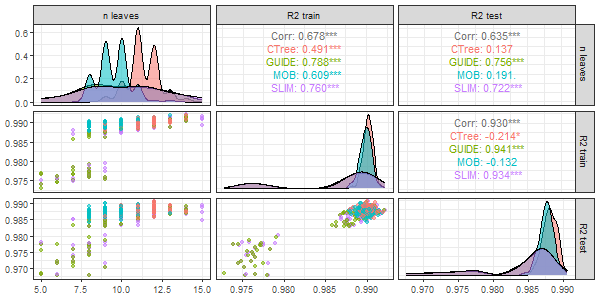
\includegraphics[width=16cm]{Figures/simulations/batchtools/basic_scenarios/linear_smooth/ls_1000_standalone_r2_nleaves.png}
    \label{fig:ls_1000_standalone_r2_nleaves}
\end{figure} 


In figure \ref{fig:ls_1000_standalone_r2_nleaves} it can be seen that, as expected, the performance accuracy increases with increasing number of leafnodes for all models. Noticeable, however, are the two different performance levels of SLIM and GUIDE for trees with $7$ to $9$ leafnodes. This is due to the fact that trees with different symmetry properties were generated by SLIM and GUIDE in this range. While in the MBTs with higher performance the distribution of the observations on the different leafnodes is approximately equal, in the group with lower performance one leaf node each was generated with almost half of the observations and the remaining half is distributed on the remaining leafnodes. This is shown in more detail in the appendix \textbf{appendix einfügen}. There one can also see that the strongly assymmetric trees with one leaf node each with the large number of observations have only just fallen short of the prepruning criterion $impr$ in this node. The choice of the parameter $impr$ therefore also has a decisive influence on the resulting tree at this point.





\begin{figure}[!htb] 
\caption{Test accuracy $R^2$ vs number of leaf nodes scenario \textbf{linear smooth} with $n=1500, alpha = 0.001, impr = 0.1$}
    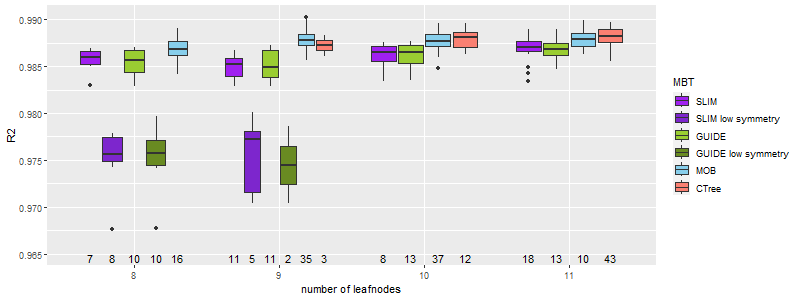
\includegraphics[width=16cm]{Figures/simulations/batchtools/basic_scenarios/linear_smooth/ls_1000_standalone_r2_test.png}
    \label{fig:ls_1000_standalone_r2_test}
\end{figure} 

Figure \ref{fig:ls_1000_standalone_r2_test} shows the accuracy depending on the number of leaf nodes for the four different MBTs.
The numbers below each box indicate how many of the $100$ trees created with each of the four algorithms have the respective number of leafnodes. For example, 8 of the 100 SLIM trees have 10 leafnodes and the corresponding box was created from these 10 results. Note that the numbers do not add up to a hundred, as there is also a small number of trees with leafnodes outside the range shown here. The results of SLIM and GUIDE are divided into two groups for 8 and 9 leafnodes for this plot. Trees with low symmetry are here defined as trees in which the largest leafnode contains at least 350 observations. The results between the two groups differ greatly, as already recognised in figure \ref{fig:ls_1000_standalone_r2_nleaves}.
The figure shows that accuracy is very high in all four MBT. Over the range shown, MOB and CTree (from number of leaves = 9) have slightly higher performance than SLIM and GUIDE with the same number of leaf nodes, i.e. MOB and CTree achieve a better trade-off between performance and interpretability in this scenario as standalone model.
As can be seen in Figure \ref{fig:app_ls_1000_standalone_symmetrie} in the appendix, SLIM and GUIDE have a higher average maximum leafsize (lower symmetrie) over the entire comparable range of leafnodes than MOB and GUIDE, which could be a reason for the slightly worse performance.
However, when the models are used as surrogate models on lm predictions, the performance of the different MBTs with the same number of leafnodes is very close (see appendix Figures \ref{fig:app_ls_1000_lm_r2_test}, \ref{fig:app_ls_1000_xgboost_r2_test})
Overall, it should  be noted that the number of leafnodes required to achieve a similar performance as the correctly specified linear model is very high, considering that it is actually a very simple data generating process. This is because the smooth interaction can only be well approximated through many binary splits. 






\begin{figure}[!htb] 
\caption{Number of leafnodes linear smooth}
    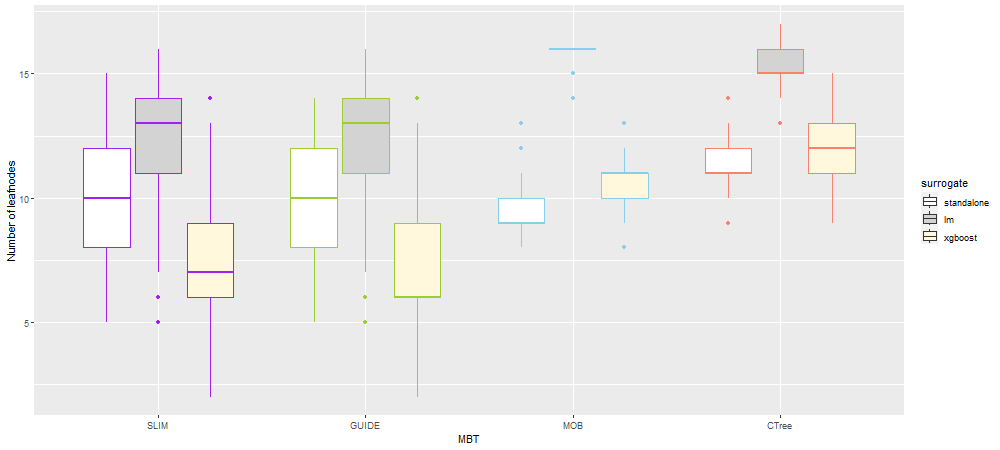
\includegraphics[width=16cm]{Figures/simulations/batchtools/basic_scenarios/linear_smooth/ls_1000_int.png}
    \label{fig:ls_1000_int}
\end{figure} 


As can be seen in figure \ref{fig:ls_1000_standalone_r2_nleaves}, the number of leaf nodes fluctuates considerably more with SLIM and GUIDE than with MOB and CTree. 
Figure \ref{fig:ls_1000_int} shows that this is also the case when the MBTs are used as surrogate models. 


\begin{figure}[!htb]
\caption{Rand Indices for scenario \textbf{linear smooth}}
    \centering
    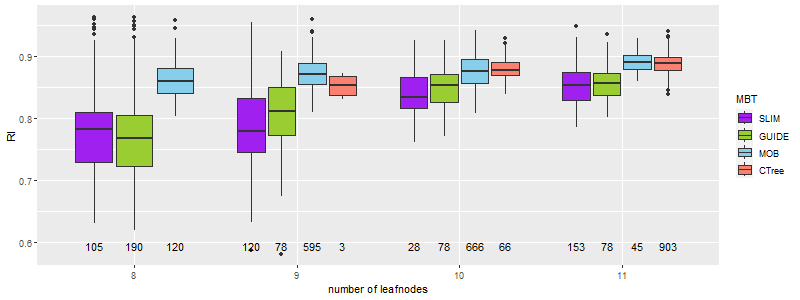
\includegraphics[width=16cm]{Figures/simulations/batchtools/basic_scenarios/linear_smooth/ls_1000_standalone_sta.png}
    \label{fig:ls_1000_standalone_sta}
\end{figure}

This observation is already a sign of lower stability of SLIM and GUIDE compared to MOB and CTree. Moreover, in figure \ref{fig:ls_1000_standalone_sta} the rand indices of the different algorithms are plotted for tree pairs with identical number of leafnodes. There you can see that even with identical numbers of leafnodes, MOB and CTree generate more stable trees.







\paragraph{Linear Categorical} 
In the linear categorical scenario, the data-generating process is not determined by a smooth interaction, but can be fully described by main effect models in four subgroups.
This would require a split at mean of the feature $x_1$ and a split with respect to the binary variable $x_3$. 
SLIM and GUIDE differ greatly from MOB and CTree in their ability to find these splits, which can be seen in Table \ref{tab:linear_abrupt_summary}. 
The column share $x_2$ indicates what proportion of all split observations were split on average with respect to the variable $x_2$.
For SLIM and GUIDE this value is $0$ for all values of $impr$ , which indicates, that the splits where performed regarding the variables $x_1$ and $x_3$.
MOB and CTree, on the other hand, split almost only with respect to the variable $x_2$ and therefore achieve a worse mean performance than SLIM and GUIDE (except for $impr = 0.15$) despite a considerable higher number of leafnodes.

\begin{table}[!htb]

\caption{Mean simulation results on 100 simulation runs as stand alone models on scenario \textbf{linear categorical} with sample size $n = 1500$ for different values of $impr$ and $alpha$}
\centering \tiny
\begin{tabular}[t]{l|r|r|r|r|r|r|r|r|r}
\hline
MBT & impr  & n leaves & n leaves min & n leaves max & $R^2_{train}$ & sd $R^2_{train}$ & $R^2_{test}$ & sd $R^2_{test}$ & share $x_2$\\
\hline

\hline
SLIM & 0.15 & 2.00 & 2 & 2 & 0.8272 & 0.0071 & 0.8250 & 0.0111 & 0.0000\\
SLIM & 0.10 & 3.99 & 3 & 4 & 0.9884 & 0.0069 & 0.9870 & 0.0078 & 0.0000\\
SLIM & 0.05 & 4.00 & 4 & 4 & 0.9891 & 0.0010 & 0.9878 & 0.0028 & 0.0000\\
GUIDE & 0.15 & 2.00 & 2 & 2 & 0.8272 & 0.0071 & 0.8250 & 0.0111 & 0.0000\\
GUIDE & 0.10 & 3.99 & 3 & 4 & 0.9884 & 0.0069 & 0.9870 & 0.0078 & 0.0000\\
GUIDE & 0.05 & 4.00 & 4 & 4 & 0.9891 & 0.0010 & 0.9878 & 0.0028 & 0.0000\\
\hline

  & alpha & & & & & & & & \\
\hline
MOB & 0.001 & 12.77 & 10 & 15 & 0.9661 & 0.0083 & 0.9558 & 0.0091 & 0.9095\\
MOB & 0.010 & 14.40 & 12 & 16 & 0.9736 & 0.0067 & 0.9641 & 0.0076 & 0.8761\\
MOB & 0.050 & 14.85 & 13 & 17 & 0.9747 & 0.0063 & 0.9654 & 0.0071 & 0.8682\\
CTree & 0.001 & 11.87 & 10 & 14 & 0.9484 & 0.0030 & 0.9390 & 0.0052 & 0.9976\\
CTree & 0.010 & 12.82 & 11 & 15 & 0.9498 & 0.0030 & 0.9404 & 0.0051 & 0.9939\\
CTree & 0.050 & 13.61 & 11 & 16 & 0.9508 & 0.0029 & 0.9411 & 0.0048 & 0.9923\\
\hline
lm & & & & & 0.9702 & 0.0018 & 0.9694 & 0.0029 &\\
xgboost & & & & & 0.9876 & 0.0015 & 0.9778 & 0.0031 & \\
\hline

\end{tabular}
\label{tab:linear_abrupt_summary} 
\end{table}



In contrast to the scenario linear smooth, the variation in the number of leafnodes for fixed values of $impr$ is also small for SLIM and GUIDE. This indicates a high stability of SLIM and CTree on this scenario. 



\begin{figure}[!htb]
\caption{Test accuracy $R^2$ vs number of leaf nodes scenario \textbf{linear categorical} with $n=1500, alpha = 0.001, impr = 0.05$}
    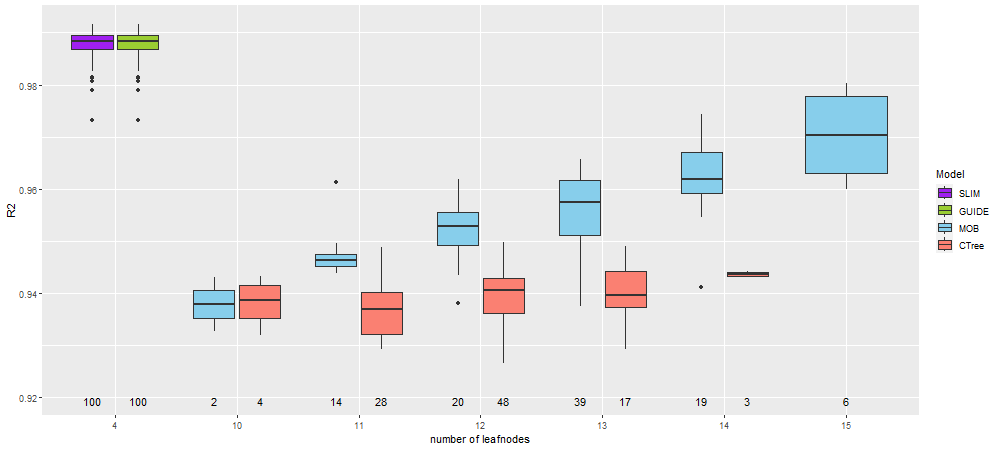
\includegraphics[width=16cm]{Figures/simulations/batchtools/basic_scenarios/linear_abrupt/la_1000_standalone_r2_test.png}
    \label{fig:la_1000_standalone_r2_test}
\end{figure} 

Figure \ref{fig:la_1000_standalone_r2_test} shows the performance by number of leafnodes for impr = 0.05 and alpha = 0.001. There one can see again that SLIM and GUIDE achieve a very high $R^2$ despite the low number of leafnodes. 

It is also noticeable that MOB performs better than CTree with the same number of leafnodes.
This could be because, according to \citep{Schlosser.2019}, the M-fluctuation test used in MOB has a higher ability in detecting abrupt changes than the linear test statistic used in CTree.




If SLIM and GUIDE are fitted as surrogate models on the predictions of a GAM (linear main effects, interaction by means of tensorproduct interaction), the number of leafnodes increases and the variability also increases. This indicates that the interactions with the GAM were not fitted well enough (despite $R^2_{test} = 0.97$ see table \ref{tab:linear_abrupt_summary}). The statement that SLIM is more stable when used as a surrogate model than when used as a standalone model \citep{Hu.2020} is therefore not true in this case.
Nevertheless, the mean performance of SLIM and GUIDE is better than that of the other MBTs, as can be seen in Table \ref{tab:app_linear_abrupt_1000} in the appendix.




\paragraph{Linear Mixed}
\begin{table}[!htb]
\caption{Mean simulation results on 100 simulation runs as stand alone models on scenario \textbf{linear mixed} with sample size $n = 1500$ for different values of $impr$ and $alpha$}
\centering \tiny
\begin{tabular}[t]{l|r|r|r|r|r|r|r|r|r}
\hline


MBT & impr  & n leaves & n leaves min & n leaves max & $R^2_{train}$ & sd $R^2_{train}$ & $R^2_{test}$ & sd $R^2_{test}$ & share $x_1$ $x_2$\\
\hline

SLIM & 0.15 & 3.40 & 2 & 11 & 0.8853 & 0.0309 & 0.8771 & 0.0336 & 0.9592\\
SLIM & 0.10 & 13.07 & 8 & 16 & 0.9801 & 0.0073 & 0.9743 & 0.0083 & 0.8793\\
SLIM & 0.05 & 14.73 & 13 & 16 & 0.9830 & 0.0019 & 0.9774 & 0.0029 & 0.8794\\
GUIDE & 0.15 & 3.29 & 2 & 11 & 0.8839 & 0.0305 & 0.8758 & 0.0329 & 0.9598\\
GUIDE & 0.10 & 12.52 & 7 & 15 & 0.9789 & 0.0087 & 0.9732 & 0.0091 & 0.8581\\
GUIDE & 0.05 & 14.19 & 12 & 16 & 0.9822 & 0.0024 & 0.9766 & 0.0032 & 0.8516\\

\hline

& alpha & & & & & & & \\
\hline

MOB & 0.001 & 14.52 & 13 & 17 & 0.9802 & 0.0017 & 0.9725 & 0.0027 & 0.9679\\
MOB & 0.010 & 14.73 & 13 & 17 & 0.9803 & 0.0017 & 0.9726 & 0.0028 & 0.9672\\
MOB & 0.050 & 14.80 & 13 & 17 & 0.9804 & 0.0017 & 0.9727 & 0.0028 & 0.9664\\

CTree & 0.001 & 14.80 & 12 & 17 & 0.9802 & 0.0017 & 0.9731 & 0.0023 & 0.9989\\
CTree & 0.010 & 14.98 & 13 & 17 & 0.9802 & 0.0017 & 0.9731 & 0.0023 & 0.9978\\
CTree & 0.050 & 15.03 & 13 & 17 & 0.9802 & 0.0017 & 0.9731 & 0.0023 & 0.9978\\
\hline

xgboost & & & & & 0.9859 & 0.0014 & 0.9682 & 0.0042 &\\
lm & & & & & 0.9902 & 0.0006 & 0.9898 & 0.0008 &\\
\hline


\end{tabular}
\label{tab:linear_mixed_summary}
\end{table}

The scenario linear mixed contains both smooth interactions that can only be handled by splits with respect to the numerical variables $\textbf{x}_1$ and $\textbf{x}_2$, and subgroups defined by the binary variables $\textbf{x}_3$ and $\textbf{x}_4$. 
The average proportion of splits carried out with respect to the two numerical variables is shown in table \ref{tab:linear_mixed_summary}.
For $alpha = 0.001$ and $impr = 0.05$ the mean number of leaf nodes is similar for all four MBT algorithms. The table shows that the average performance of SLIM and GUIDE for this setting is on average higher than that of the other two MBTs and at the same time the mean proportion of splits with respect to the numerical variable is lower.  This means that SLIM and GUIDE use the binary variables more often to reveal the subgroups defined by them, while MOB and even more pronounced CTree split almost exclusively along the numerical features and thus perform worse despite having the same mean number of leafnodes. 

In this example, SLIM and GUIDE achieve a better tradeoff between performance and interpretability than MOB and CTree.


In the figures \ref{fig:lm_1000_standalone_r2_test}  and \ref{fig:lm_1000_standalone_share_x3x4} this is broken down in more detail.


\begin{figure}[!htb]
\caption{Test accuracy $R^2$ vs number of leaf nodes scenario \textbf{linear mixed} with $n=1500, alpha = 0.001, impr = 0.05$}
    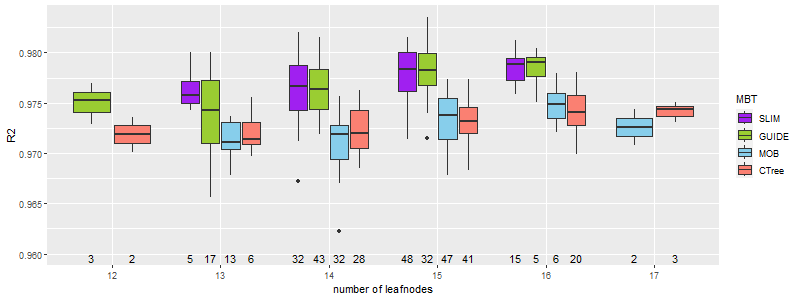
\includegraphics[width=16cm]{Figures/simulations/batchtools/basic_scenarios/linear_mixed/lm_1000_standalone_r2_test.png}
    \label{fig:lm_1000_standalone_r2_test}
\end{figure} 


\begin{figure}[!htb]
\caption{Share of splitted observations by features $\textbf{x}_3, \textbf{x}_4$ vs number of leaf nodes scenario linear mixed with $n=1500, alpha = 0.001, impr = 0.05$}
    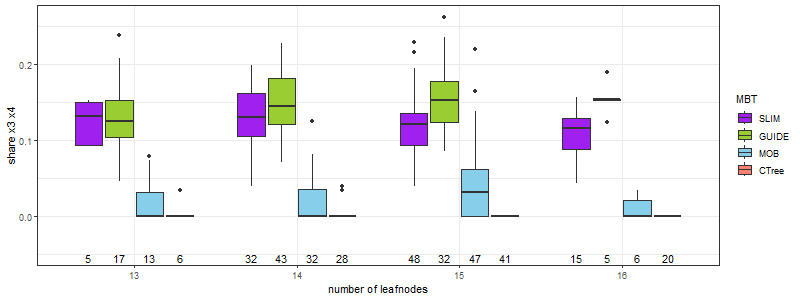
\includegraphics[width=16cm]{Figures/simulations/batchtools/basic_scenarios/linear_mixed/lm_1000_standalone_share_x3x4.png}
    \label{fig:lm_1000_standalone_share_x3x4}
\end{figure} 




\begin{figure}[!htb]
\caption{Rand Indices for scenario linear mixed}
    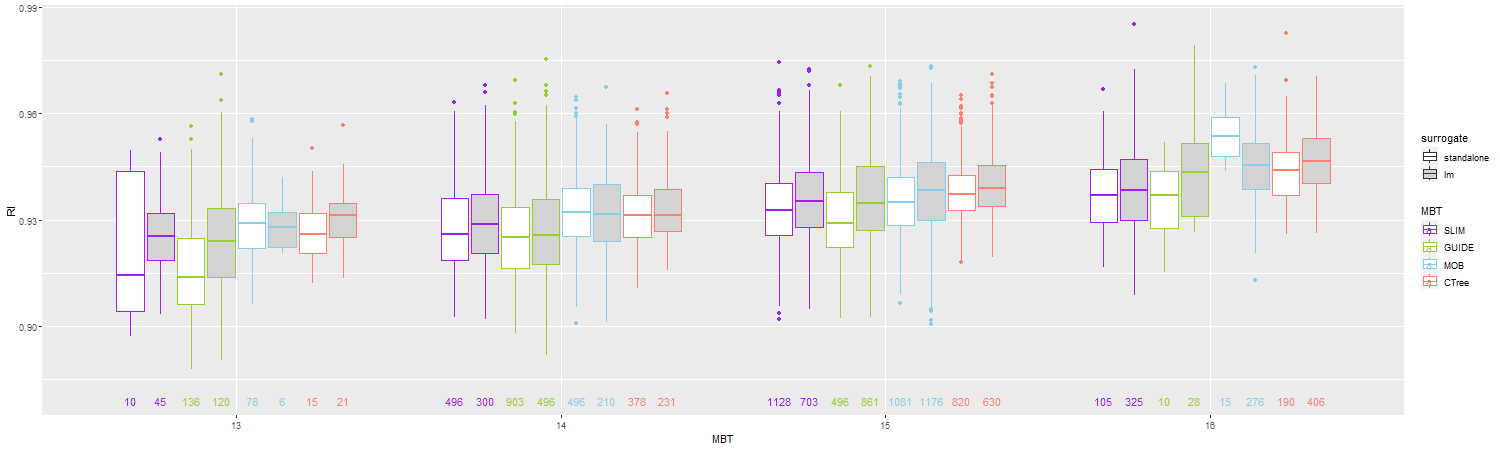
\includegraphics[width=16cm]{Figures/simulations/batchtools/basic_scenarios/linear_mixed/lm_1000_standalone_lm_sta.png}
    \label{fig:lm_1000_standalone_lm_sta}
\end{figure}

For the comparison of stability we look at figure \ref{fig:lm_1000_standalone_lm_sta}. On the one hand, it can be seen that MOB and CTree seem to be somewhat more stable than SLIM and GUIDE with the same number of leafnodes, but the difference is not great. Furthermore, it can be seen that in most cases the stability of trees with the same number of leafnodes is higher when they are used as surrogates than when they are used as standalone models. Here, the assertion of \citep{Hu.2020} that SLIM is more stable when used as a surrogate is true and also applies to the other algorithms.


\newpage
\subsection{Linear smooth with correlated features}
While in the basic scenarios the features were independent of each other, this scenario examines how a correlations between features influence the MBTs. For this purpose, the "linear smooth" scenario is modified so that there is a correlation between $x_1$ and $x_3$.
\begin{itemize}
    \item $\textbf{x}_1,..., \textbf{x}_3 \sim U(-1,1), Corr(\textbf{x}_1, \textbf{x}_3) = \rho_{13} \in {0.1, 0.5, 0.9}$
    \item $ f_{ls}(\textbf{x}) = \textbf{x}_1 + 4   \textbf{x}_2 + 3   \textbf{x}_2   \textbf{x}_3 $
    \item $\epsilon \sim N(0, 0.1 sd(f_{ls}(x))$
    \item $y = f_{ls}(\textbf{x}) + \epsilon$
\end{itemize}

              
It is to be examined whether the modification causes the feature $\textbf{x}_1$ to be incorrectly selected as a splitting variable.


For the simulation, the MBTs are fitted on a dataset with sample size $ n = 1500$ ($1000$ training, $500$ test observations) using the pruning parameter settings $alpha = 0.001$ and $impr = 0.01$. The parameters were chosen so that the average number of leafnodes is similar for the different MBTs. The trees are fitted both as standalone models on the original data and as surrogate models on correctly specified linear models. The simulation is repeated $250$ times.


\begin{table}[!htb]
\caption{mean results correlated data}
\centering \tiny
\begin{tabular}[t]{l|l|r|r|r|r|r|r|r|r|r}
\hline
black nox & MBT & $\rho_{13}$ & $x_1$ frequency & n leaves & n leaves min & n leaves max & $R^2_{train}$  & sd $R^2_{train}$ & $R^2_{test}$ & sd $R^2_{test}$ \\
\hline
standalone & SLIM & 0.1 & 0.088 & 10.012 & 3 & 16 & 0.9863 & 0.0055 & 0.9836 & 0.0061\\
standalone & SLIM Ridge & 0.1 & 0.096 & 9.756 & 4 & 15 & 0.9860 & 0.0057 & 0.9834 & 0.0063\\
standalone & GUIDE & 0.1 & 0.052 & 9.792 & 3 & 15 & 0.9862 & 0.0057 & 0.9836 & 0.0061\\
standalone & MOB & 0.1 & 0.000 & 9.392 & 8 & 12 & 0.9898 & 0.0006 & 0.9876 & 0.0010\\
standalone & CTree & 0.1 & 0.000 & 11.312 & 9 & 14 & 0.9901 & 0.0006 & 0.9881 & 0.0010\\
\hline
standalone & SLIM & 0.5 & 0.152 & 10.052 & 3 & 15 & 0.9867 & 0.0050 & 0.9841 & 0.0055\\
standalone & SLIM Ridge & 0.5 & 0.112 & 9.612 & 3 & 15 & 0.9862 & 0.0051 & 0.9837 & 0.0056\\
standalone & GUIDE & 0.5 & 0.120 & 9.776 & 3 & 15 & 0.9870 & 0.0046 & 0.9846 & 0.0052\\
standalone & MOB & 0.5 & 0.000 & 9.048 & 8 & 11 & 0.9899 & 0.0006 & 0.9878 & 0.0010\\
standalone & CTree & 0.5 & 0.000 & 10.776 & 9 & 14 & 0.9901 & 0.0006 & 0.9882 & 0.0010\\
\hline
standalone & SLIM & 0.9 & 0.328 & 10.216 & 4 & 16 & 0.9873 & 0.0043 & 0.9850 & 0.0046\\
standalone & SLIM Ridge & 0.9 & 0.292 & 9.968 & 4 & 16 & 0.9872 & 0.0043 & 0.9848 & 0.0048\\
standalone & GUIDE & 0.9 & 0.448 & 9.996 & 3 & 17 & 0.9874 & 0.0042 & 0.9852 & 0.0047\\
standalone & MOB & 0.9 & 0.048 & 8.704 & 8 & 11 & 0.9899 & 0.0005 & 0.9879 & 0.0010\\
standalone & CTree & 0.9 & 0.084 & 10.280 & 8 & 14 & 0.9901 & 0.0005 & 0.9882 & 0.0009\\
\hline
lm & SLIM & 0.1 & 0.000 & 12.060 & 5 & 16 & 0.9967 & 0.0047 & 0.9959 & 0.0055\\
lm & SLIM Ridge & 0.1 & 0.000 & 11.388 & 5 & 16 & 0.9962 & 0.0049 & 0.9954 & 0.0057\\
lm & GUIDE & 0.1 & 0.000 & 12.132 & 5 & 16 & 0.9967 & 0.0047 & 0.9960 & 0.0055\\
lm & MOB & 0.1 & 0.000 & 15.764 & 14 & 16 & 0.9994 & 0.0001 & 0.9993 & 0.0001\\
lm & CTree & 0.1 & 0.000 & 15.256 & 13 & 17 & 0.9993 & 0.0001 & 0.9992 & 0.0001\\
\hline
lm & SLIM & 0.5 & 0.000 & 12.008 & 5 & 16 & 0.9970 & 0.0042 & 0.9963 & 0.0050\\
lm & SLIM Ridge & 0.5 & 0.000 & 11.584 & 4 & 16 & 0.9967 & 0.0043 & 0.9960 & 0.0051\\
lm & GUIDE & 0.5 & 0.000 & 11.968 & 5 & 16 & 0.9974 & 0.0036 & 0.9968 & 0.0043\\
lm & MOB & 0.5 & 0.000 & 15.768 & 14 & 16 & 0.9995 & 0.0001 & 0.9994 & 0.0001\\
lm & CTree & 0.5 & 0.000 & 15.220 & 13 & 17 & 0.9994 & 0.0001 & 0.9993 & 0.0001\\
\hline
lm & SLIM & 0.9 & 0.000 & 12.212 & 5 & 16 & 0.9977 & 0.0033 & 0.9972 & 0.0039\\
lm & SLIM Ridge & 0.9 & 0.000 & 11.772 & 5 & 16 & 0.9975 & 0.0034 & 0.9970 & 0.0039\\
lm & GUIDE & 0.9 & 0.000 & 12.364 & 5 & 16 & 0.9978 & 0.0033 & 0.9973 & 0.0038\\
lm & MOB & 0.9 & 0.004 & 15.752 & 14 & 17 & 0.9996 & 0.0001 & 0.9995 & 0.0001\\
lm & CTree & 0.9 & 0.000 & 15.144 & 14 & 17 & 0.9995 & 0.0001 & 0.9994 & 0.0001\\
\hline
\end{tabular}
\label{tab:linear_smooth_correlated_summary}
\end{table} 


Table \ref{tab:linear_smooth_correlated_summary} shows the average performance and the number of leaf nodes of MBTs  as well as the proportion of trees "freq $\textbf{x}_1$" where $\textbf{x}_1$ is wrongly chosen as the splitting variable.
If the MBTs are used as standalone, SLIM and GUIDE choose feature $\textbf{x}_1$ as splitting variable already at a very low correlation of 0.1 in some cases. As the correlation increases, this frequeny increases. MOB and CTree, on the other hand, only use the variables actually involved in the interaction for the splits at $\rho \in \{0.1, 0.5\}$, but at a very high correlation $rho = 0.9$ they also include $x_1$ for the split in a small number of cases. 
Since the use of ridge regression for correlated features is becoming more common, SLIM was also fitted with ridge regression models in the nodes. The choice of the penalization parameter is made in each recursion step by minimising the BIC. Instead of the SSE, the penalised SSE is used as objective function. However, this does not result in any systematic improvement. 
If the MBTs are used as surrogates for the lm predictions instead of standalone models, there are hardly any false splits in this scenario. So it seems that the problem of correlated features is reduced when the models are used as surrogates.


\subsection{Linear smooth with noise features}
This scenario examines how noise features that have no influence on $y$ affect the MBTs. Here, again, the scenario linear smooth was used as a basis, to which six noise variables were added.
In addition to the usual models, SLIM models were fitted with LASSO regression models. LASSO models allow the fitting of sparse models, i.e. a feature selection in the nodes takes place automatically.The strength of the feature selection depends strongly on the penalisation parameter. Three different variants were used to choose this parameter. In all SLIM LASSO MBTs, the penalisation parameter was selected using the BIC criterion. However, in the case of $df = 3$ or $df = 2$, the additional restriction was defined that the effective degrees of freedom must not exceed this value. This enforces especially sparse models.

\begin{itemize}
    \item $\textbf{x}_1,..., \textbf{x}_{10} \sim U(-1,1)$
    \item $ f_{ls}(\textbf{x}) = \textbf{x}_1 + 4   \textbf{x}_2 + 3   \textbf{x}_2   \textbf{x}_3 $
    \item $\epsilon \sim N(0, 0.1 \cdot sd(f_{ls}(x))$
    \item $y = f_{ls}(\textbf{x}) + \epsilon$
\end{itemize}

This examines whether the noise variables are incorrectly used as splitting variables.
As in the previous scenario the MBTs are fitted as standalone models and surrogates on lm predictions on a dataset with sample size $ n = 3000$ ($2000$ training, $1000$ test observations) using the pruning parameter settings $alpha = 0.001$ and $impr = 0.1$. The simulation is repeated $250$ times.

\begin{table}[!htb]
\caption{Mean simulation results as stand alone model and as surrogate on lm predictions on scenario Linear smooth with noise features}
\centering \tiny
\begin{tabular}[t]{l|l|r|r|r|r|r|r|r|r|r}
\hline
black box & MBT & freq $ \textbf{x}_{noise}$  & share $\textbf{x}_3$ & n leaves & n leaves min & n leaves max & $R^2_{train}$  & sd $R^2_{train}$ & $R^2_{test}$ & sd $R^2_{test}$\\
\hline
standalone & SLIM & 0.072 & 0.4654 & 11.988 & 5 & 17 & 0.9880 & 0.0048 & 0.9854 & 0.0049\\
standalone & SLIM LASSO & 0.092 & 0.4655 & 11.048 & 5 & 16 & 0.9871 & 0.0049 & 0.9852 & 0.0051\\
standalone & SLIM LASSO df 3 & 0.028 & 0.5182 & 9.732 & 4 & 14 & 0.9863 & 0.0046 & 0.9848 & 0.0050\\
standalone & SLIM LASSO df 2 & 0.028 & 0.9990 & 9.648 & 4 & 15 & 0.9864 & 0.0044 & 0.9852 & 0.0047\\
standalone & GUIDE & 0.104 & 0.4780 & 11.788 & 5 & 16 & 0.9880 & 0.0047 & 0.9854 & 0.0048\\
standalone & MOB & 0.000 & 0.5038 & 11.096 & 8 & 14 & 0.9901 & 0.0005 & 0.9878 & 0.0007\\
standalone & CTree & 0.000 & 0.5087 & 13.140 & 10 & 16 & 0.9904 & 0.0004 & 0.9882 & 0.0007\\
\hline

standalone & lm & & & & & & 0.9901 & 0.0004 & 0.9901 & 0.0006\\

\hline
lm & SLIM & 0.000 & 0.4900 & 14.036 & 8 & 16 & 0.9987 & 0.0018 & 0.9984 & 0.0019\\
lm & SLIM LASSO & 0.000 & 0.4574 & 13.736 & 8 & 16 & 0.9985 & 0.0023 & 0.9982 & 0.0027\\
lm & SLIM LASSO df 3 & 0.000 & 0.5076 & 14.008 & 8 & 16 & 0.9985 & 0.0023 & 0.9983 & 0.0026\\
lm & SLIM LASSO df 2 & 0.000 & 1.0000 & 11.160 & 5 & 14 & 0.9979 & 0.0018 & 0.9977 & 0.0020\\
lm & GUIDE & 0.000 & 0.4909 & 14.096 & 8 & 16 & 0.9988 & 0.0018 & 0.9984 & 0.0019\\
lm & MOB & 0.000 & 0.5073 & 15.960 & 15 & 16 & 0.9995 & 0.0000 & 0.9993 & 0.0001\\
lm & CTree & 0.000 & 0.5003 & 15.564 & 13 & 16 & 0.9994 & 0.0001 & 0.9992 & 0.0001\\
\hline
\end{tabular}
\label{tab:linear_smooth_noisy_summary}
\end{table}

Table \ref{tab:linear_smooth_noisy_summary} shows the mean simulation results. freq $ \textbf{x}_{wrong}$ is the proportion of trees in which at least one of the noise variables was used as a splitting variable. 
As in the correlated data scenario, wrong variables are only used as splitting variables for the specified settings if the MBTs are used as standalone models. However, MOB and CTree do not select false variables even then. For the SLIM MBTs it can be seen that freq $\textbf{x}_{wrong}$ decreases with a strong penalty (df = 2 and df = 3). GUIDE, on the other hand, has the most problems with the noise variables and the highest value for freq $x_{wrong}$.
An interesting effect of using a LASSO model with a maximum of 2 effective degrees of freedom is that for the splitting almost exclusively variable $\textbf{x}_3$ is used, although otherwise $\textbf{x}_2$ and $\textbf{x}_3$ are mostly chosen similarly often. This could be because $\textbf{x}_3$ does not have a main effect on the response, but $\textbf{x}_2$ and $\textbf{x}_1$ do.  Due to the strong penalisation, only these two features are used for modelling in the leafs. Since $\textbf{x}_3$ is not included in the modelling, it is instead more often used as a splitting variable.
The interpretability of this MBT is thus increased on the one hand by the very sparse models in the leaf nodes and on the other hand by the fact that the splits are almost only carried out with respect to $\textbf{x}_3$, which is easier to keep track of than if the feature space is split with respect to several different variables.
The average number of leafnodes for SLIM with LASSO df 2 is smaller than for the standard SLIM MBT, which is why the performance cannot be directly compared.  However, it can be seen that the training performance of SLIM with LASSO df 2 is further below that of the standard SLIM than the test performance. This means that with the strong penalisation, the overfitting can also be reduced.
In the appendix in the figures \ref{fig:app_lasso_standalone_r2_test} and \ref{fig:app_lasso_standalone_r2_test_slim} there is a more detailed presentation of the individual results. It is particularly noticeable that, as with the basic scenario linear smooth, all SLIM MBTs and GUIDE generate some strongly asymmetrical trees, which then have a considerable poorer performance.




\subsection{Non-linear Effects}
While the main goal so far has been to compare the different MBT algorithms on simple scenarios with linear maineffects, the following scenario will investigate how the choice of different objective functions affects the interpretability and performance of SLIM MBTs when non-linear maineffects enter the data generating process. 
As it is very flexible in the selection of the objective, only the SLIM algorithm is used.

\begin{itemize}
    \item $\textbf{x}_1, ..., \textbf{x}_5 \sim U(-1,1)$, $\textbf{x}_6 \sim Bern(0.5)$, 
    \item $ f_{nl}(\textbf{x}) = \textbf{x}_1 + 2 \textbf{x}_2^2 + \textbf{x}_3log(abs(\textbf{x}_3)) + \textbf{x}_4\textbf{x}_5 + \textbf{x}_1\textbf{x}_4\mathbf{I}_{\textbf{x}_6 = 0}$
    \item $\epsilon \sim N(0,  0.1 \cdot sd(f_{nl}(x))$
    \item $y = f_{nl}(\textbf{x}) + \epsilon$     
\end{itemize}

SLIM is fitted here with four different objectives.
\begin{enumerate}
    \item linear regression model (lm)
    \item polynomial regression of degree $2$ with LASSO penalization (penalized poly)
    \item linear regression with linear bspline transformations of the features (bsplines)
    \item Generalized additive models with integrated smoothness estimation \citep{Wood.2011} (GAM)
\end{enumerate}


Since the models in the leafnodes are of different complexity for different objectives, it is not sufficient in this case to use only the number of leafnodes as a measure of interpretability. In addition, the following criteria are considered:
\begin{itemize}
    \item effective degrees of freedoms of the leaf node models (lm and penalized poly), as sparse models are easier to interpret
    \item proportion of observation splits where the split is actually due to an interaction rather than an incompletely modelled main effect
    \item interpretable weights versus merely visually interpretability
\end{itemize}

In order to enable a comparison of the interpretability, the $R^2$ is used for prepruning in this scenario in addition to the prepruning by means of minimum loss reduction. As soon as the $R^2$ exceeds a certain value in a node, it is no longer split. 

Three different settings were simulated
\begin{table}[!htt]
    \centering
    \begin{tabular}{l|r|r}
        \hline
        scenario  &  impr & $R^2$ \\
        \hline
        scenario 1 & 0.05 & 0.9 \\
        scenario 2 & 0.05 & 0.95 \\
        scenario 3 & 0.10 & 1  \\
        \hline

    \end{tabular}
    \caption{simulation setting nonlinear}
    \label{tab:}
\end{table}

For all three scenarios a sample size of 3000 is used and the simulation is repeated 50 times. The MBTs are fitted both as standalone models and as surrogate models on predictions of an xgboost model.


\begin{table}[!htb]

\caption{mean interpretability simulation results nonlinear scenario 1}
\centering \tiny
\begin{tabular}[t]{l|l|r|r|r|r|r|r|r|r|r}
\hline
black box & model & n leaves & n l min & n l max & n split feat & n sf min & n sf max & \% main effect & df & sd df\\
\hline
standalone & lm & 17.48 & 13 & 28 & 4.76 & 4 & 6 & 0.4525 & 6.5763 & 0.1578\\
standalone & penalized poly & 4.36 & 3 & 7 & 2.16 & 2 & 3 & 0.3605 & 8.1847 & 0.8960\\
standalone & bsplines & 2.04 & 2 & 3 & 1.00 & 1 & 1 & 0.0000 &  & \\
standalone & gam & 2.04 & 2 & 3 & 1.00 & 1 & 1 & 0.0000 &  & \\
\hline
xgboost & lm & 19.82 & 2 & 33 & 4.76 & 1 & 6 & 0.6125 & 6.8671 & 0.1438\\
xgboost & penalized poly & 3.58 & 2 & 7 & 2.08 & 1 & 4 & 0.3880 & 8.5499 & 1.1147\\
xgboost & bsplines & 1.86 & 1 & 3 & 0.84 & 0 & 1 & 0.0000 &  & \\
xgboost & gam & 1.90 & 1 & 4 & 0.88 & 0 & 2 & 0.0000 &  & \\

\hline
\end{tabular}
\label{tab:linear_mixed_1_interpretability}

\end{table}

Table \ref{tab:linear_mixed_1_interpretability} lists the mean results regarding the interpretability of the different MBTs for scenario 1, in which the prepruning in a node already applies at an $R^2$ of 0.9. For SLIM with linear regression models in the nodes, this results in very large trees which can hardly be used for interpretation purposes.
In addition, in average $45\%$ ($61\%$ if used as surrogate) of all split observations were not split with respect to an interaction, but with respect to an insufficiently modelled maineffect. Moreover, in some simulation runs all features are used as splitting variables, which further increases the lack of interpretability.
The fact that the models in the leaf nodes are very simple can hardly compensate for this. 

SLIM in conjunction with penalised polynomial regression in the nodes, on the other hand, achieves comparable performance with far fewer splits.
There are also considerable fewer different features used for splitting, but the proportion of observations where the splits were performed with respect to a main effect variable is still high, albeit better than with SLIM lm.

Both SLIM with linear bspline transformed variables and GAMs require on average only two leafnodes, i.e. one split, to achieve an $R^2$ of $0.9$. The models in the leafnodes can only be interpreted visually, but since the number of models is very small, the degree of interpretability is comparatively high. Moreover, these models actually only split by interactions, as the non-linear main effects are already modelled sufficiently well. If it is not explicitly required that the model weights are directly interpretable and it should also be ensured that they are actually split according to interactions, models with splines are the best choice in this case. GAMs are preferable to unpenalised bsplines in terms of their generalisation error, but the computational effort is much higher.




\begin{table}[!htb]

\caption{mean performance simulation results nonlinear scenario 1}
\centering \tiny
\begin{tabular}[t]{l|l|r|r|r|r|r}
\hline
black box & MBT & R2 train & R2 train sd & R2 test & R2 test sd & time\\
\hline
standalone & lm & 0.9243 & 0.0062 & 0.9113 & 0.0054 & 53.9438\\
standalone & penalized poly & 0.9204 & 0.0092 & 0.9161 & 0.0108 & 46.6282\\
standalone & bsplines & 0.9282 & 0.0036 & 0.9195 & 0.0049 & 15.2456\\
standalone & gam & 0.9253 & 0.0034 & 0.9226 & 0.0048 & 417.2874\\
\hline
xgboost & lm & 0.9200 & 0.0228 & 0.9023 & 0.0190 & 55.7771\\
xgboost & penalized poly & 0.9213 & 0.0079 & 0.9150 & 0.0087 & 35.4093\\
xgboost & bsplines & 0.9382 & 0.0118 & 0.9296 & 0.0120 & 11.4670\\
xgboost & gam & 0.9348 & 0.0118 & 0.9289 & 0.0117 & 384.7403\\
\hline
xgboost & xgboost & 0.9386 & 0.0295 & 0.9199 & 0.0362 & 3.1163\\
\hline
\end{tabular}
\end{table}




\begin{table}

\caption{mean interpretability simulation results nonlinear scenario 3}
\centering \tiny
\begin{tabular}[t]{l|l|r|r|r|r|r|r|r|r|r}
\hline
black box & model & n leaves & n l min & n l max & n split feat & n sf min & n sf max & \% main effect & df & sd df\\
\hline
standalone & basic lm & 43.06 & 36 & 48 & 5.68 & 4 & 6 & 0.5089 & 6.5804 & 0.1249\\
standalone & penalized poly & 19.32 & 16 & 22 & 4.26 & 3 & 5 & 0.2374 & 8.8768 & 0.3681\\
standalone & bsplines & 18.38 & 13 & 22 & 4.26 & 3 & 6 & 0.0126 & & \\
standalone & gam & 17.60 & 12 & 22 & 3.44 & 2 & 4 & 0.0007 & & \\
\hline
xgboost & basic lm & 30.38 & 2 & 47 & 4.56 & 1 & 6 & 0.6732 & 6.8519 & 0.1558\\
xgboost & penalized poly & 20.66 & 16 & 24 & 4.70 & 3 & 6 & 0.2327 & 9.2909 & 0.4347\\
xgboost & bsplines & 17.38 & 2 & 25 & 4.70 & 1 & 6 & 0.0597 & &\\
xgboost & gam & 15.28 & 2 & 24 & 4.00 & 1 & 6 & 0.0191 & &\\
\hline
\end{tabular}
\end{table}


\begin{table} \small

\caption{mean performance simulation results nonlinear scenario 3}
\centering
\begin{tabular}[t]{l|l|r|r|r|r|r}
\hline
black box & model & $R^2_{train}$  & sd $R^2_{train}$ & $R^2_{test}$ & sd $R^2_{test}$ & time in sec\\
\hline
standalone & basic lm & 0.9633 & 0.0035 & 0.9469 & 0.0048 & 102.2842\\
standalone & penalized poly & 0.9824 & 0.0015 & 0.9781 & 0.0020 & 195.4385\\
standalone & bsplines & 0.9929 & 0.0013 & 0.9714 & 0.0029 & 113.2447\\
standalone & gam & 0.9880 & 0.0016 & 0.9835 & 0.0017 & 1544.3393\\
\hline
xgboost & basic lm & 0.9198 & 0.0516 & 0.9030 & 0.0417 & 72.3790\\
xgboost & penalized poly & 0.9750 & 0.0033 & 0.9634 & 0.0051 & 206.5870\\
xgboost & bsplines & 0.9865 & 0.0141 & 0.9591 & 0.0092 & 97.9321\\
xgboost & gam & 0.9786 & 0.0127 & 0.9672 & 0.0115 & 1728.6021\\
\hline
xgboost & xgboost & 0.9392 & 0.0342 & 0.9216 & 0.0405 & 3.0131\\
\hline
\end{tabular}
\end{table}








